\section{Approach}
\label{sec:approach}

In this section, we describe the model which learns the word embeddings 
for cause and effect role simultaneously in an unsupervised fashion. 

\subsection{Causal Corpus Extraction}
We extract sentences containing causal knowledge by matching the 
causal patterns proposed by Luo et al.~\shortcite{luo2016commonsense}, 
such as those shown in Table~\ref{tab:cue}. 
One candidate sentence with $m+n+k$ words where $m$ is the length of cause span, $n$ is the length of effect span and $k$ is the length of causal cue, is denoted as sequence $S = \langle w_1, ..., w_m, w_1, \dots, w_k, w_1, \dots, w_n\rangle$. Causal cue splits the sentence into a cause span and an effect span, 
which is called a causal span pair collectively.  
For example~\ref{eg:sen} in Section~\ref{sec:intro}, 
the verb ``cause(d)'' is the causal cue which splits the sentence 
as follows:\\

\begin{enumerate}[(1)]
\item \underline{In 1998 the Pont du Gard was hit by major}  \underline{flooding which} [\emph{cause span}] \textbf{caused}  [\emph{causal cue}] \underline{widespread damage in the area.} [\emph{effect span}]\\
\item \underline{Rainfall is occurring as heavy downpours that} [\emph{cause span}] {\bf cause} [\emph{causal cue}] \underline{flooding.} [\emph{effect span}]
\end{enumerate}

\begin{table}[th]
	\centering
	\caption{Selected Causal cues. \textit{A} is cause span, and \textit{B} is effect span.}
	\label{tab:cue}
	\resizebox {0.45\textwidth}{!}{
		\begin{tabular}{|l l l|}
			\hline \multicolumn{3}{|c|}{intra-sentence}\\
			\hline \hline
			A lead to B & A leads to B & A led to B \\
			A give rise to B & A gives rise to B & A gave rise to B \\
			A induce B & A induces B & A induced B \\
			A cause B & A causes B & A caused B \\
			A bring on B & A brings on B & A brought on B\\
			\hline
			\multicolumn{3}{|c|}{inter-sentence}\\
			\hline \hline
			If A, then B & B because of A & B, because A \\
			A, thus B & A, therefore B & In consequence of A, B \\
			Due to A, B & B owing to A & Owing to A, B\\
			In consequence of A, B & B in consequence of A & As a consequence of A, B \\
			B as a consequence of A & A and consequently B & A , consequently B \\
			\hline
	\end{tabular}}
\end{table}

%We thus obtain two causal span pairs: (``In 1998 the Pont du Gard was hit by major flooding which'', ``widespread damage in the area.'') and (``Rainfall is occurring as heavy downpours that'', ``flooding.'').

We also consider the situation where one word alone is insufficient for
describing a complete event, such as ``give up'' in sentence 
``Don't \emph{give up} on love because of a bad experience with a 
sleazy internet site.'' Verbal phrases are included in our vocabulary 
and we use fuzzy match in the corpus to catch ``give up'' from ``give it up''.

\subsection{Vector Representation} 
\label{subsec:vec repre}

\begin{figure*}[!th]
	\centering
	%\epsfig{file=causalnet.eps, width=0.6\columnwidth}
	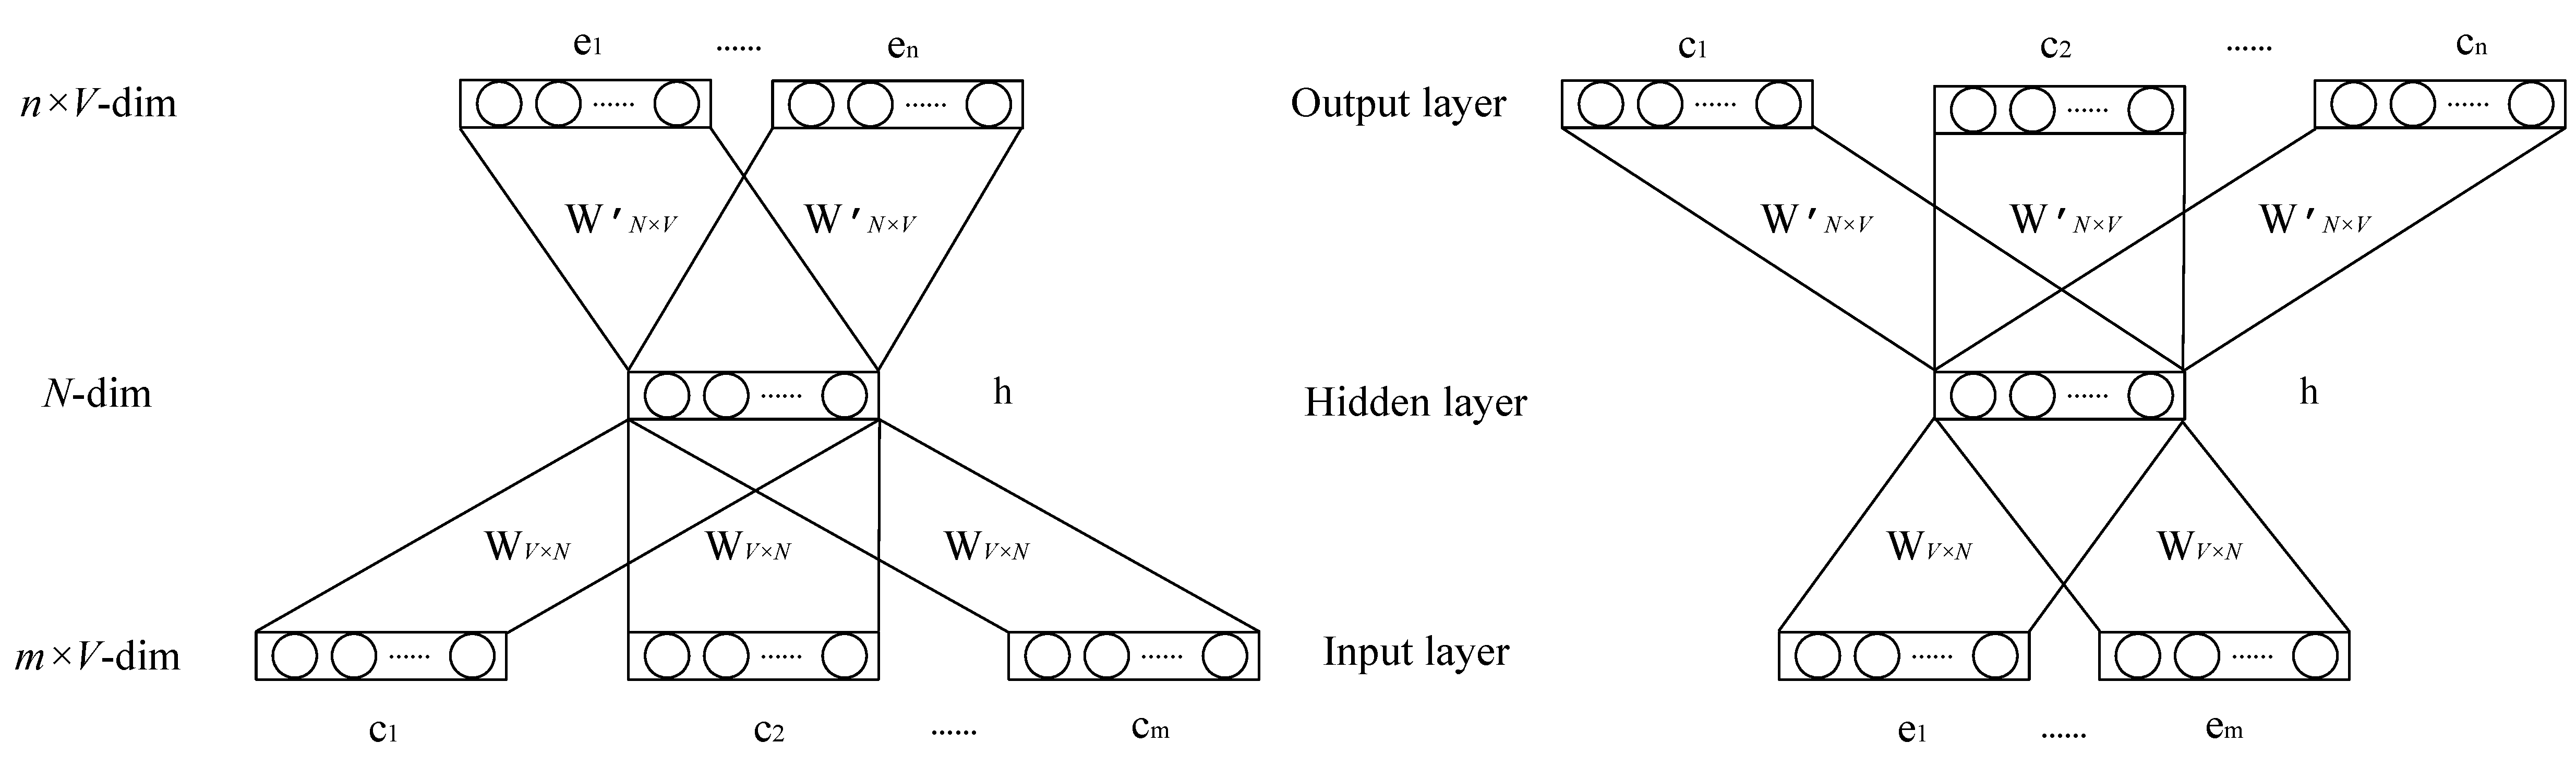
\includegraphics[width=2\columnwidth]{figure/model}
	\caption{Model of Causal Embedding}
	\label{fig:model}
\end{figure*}

We modify the idea of word2vec \cite{mikolov2013distributed} by using cause span to predict the relative effect span and vice versa(model structures are shown in Figure~\ref{fig:model}). Specifically, for word $w_i$, vector representation for cause role of $w_i$ is denoted as $\overrightarrow{c_i}$ and vector for effect role is denoted as $\overrightarrow{e_i}$. For any causal span pair, we use $C_{1 \sim m}$  and $E_{1 \sim n}$  to represent the context of cause and effect span. And the corresponding vector representations are $\overrightarrow{C_{1 \sim m}}$ and  $\overrightarrow{E_{1 \sim n}}$ where 

\begin{subequations}
	\label{eqs:contextRep}
	\begin{sequation}
	\overrightarrow{C_{1 \sim m}} = \frac{1}{m} \sum_{i=1}^m{\overrightarrow{c_i}}
	\end{sequation}
	\begin{sequation}
	\overrightarrow{E_{1 \sim n}} = \frac{1}{n} \sum_{i=1}^n{\overrightarrow{e_i}}
	\end{sequation}
\end{subequations}

We choose the straightforward way to represent span by averaging all word vectors in the span, which was a practice in the CBOW model of Word2vec as well.
As introduced by Luo~\shortcite{luo2016commonsense}, 
causality between events appear in two directions: sufficiency and necessity. 
In example~\ref{eg:sen}, causal pair (\emph{flooding}, \emph{damage}) 
encodes more of sufficiency causality because the effect \emph{damage} 
can happen not only due to \emph{flooding} but also other causes. 
Similarly, causal pair (\emph{rainfall}, \emph{flooding}) encodes more 
of necessity causality.

Suppose a sentence $S$ matches a causal cue and contains both a cause span
and an effect span. Then the probability that $S$ encodes necessity causality
is given by \eqref{eqs:prob-n} while the probability that it encodes 
sufficiency causality is given by \eqref{eqs:prob-s}.  
To simplify the problem, we suppose that \emph{all words of the other 
span are generated independently}. 

\begin{subequations}
	\begin{sequation}
	\label{eqs:prob-n}
		\begin{aligned}
			P_{nec}(S) &= P(C_{1 \sim m}|E_{1 \sim n})\\
			&= P(c_1, c_2, ..., c_m|E_{1 \sim n}) = \prod_{i=1}^{m}{P(c_i|E_{1 \sim n})}  \\
		\end{aligned}
	\end{sequation}
	\begin{sequation}
	\label{eqs:prob-s}
		\begin{aligned}
			P_{suf}(S) &= P(E_{1 \sim n}|C_{1 \sim m})\\
			&= P(e_1, e_2, ..., e_n|C_{1 \sim m}) = \prod_{j=1}^{n}{P(e_j|C_{1 \sim m})} \\
		\end{aligned}
	\end{sequation}
\end{subequations}


Inspired by CBOW in word2vec and negative sampling, we define the
objective function for training as follows:
\begin{subequations}
	\label{eqs:loss}
	\begin{sequation}
	\label{eqs:loss_suf}
	\begin{aligned}
		\max \,\, &l_{suf} = -\log P_{suf}(S) = - \sum_{j=1}^{n}{\log P(e_j|C_{1 \sim m})} \\
		&= - \sum_{j=1}^{n}{\log \frac{exp(\overrightarrow{e_j} \cdot \overrightarrow{C_{1 \sim m}} )}{\sum_{w=1}^{W}{exp(\overrightarrow{e_w} \cdot \overrightarrow{C_{1 \sim m}})}}} \\
		&= -\sum_{j=1}^{n}{[\log\sigma(\overrightarrow{e_j} \cdot \overrightarrow{C_{1 \sim m}})} + \sum_{k=1}^{K}{\log(1 - \sigma(\overrightarrow{e_k} \cdot \overrightarrow{C_{1 \sim m}}))}]\\	
	\end{aligned}
	\end{sequation}
	\begin{sequation}
		\label{eqs:loss_nec}
		\begin{aligned}
		\max \,\, &l_{nec} = -\log P_{nec}(S) = -\sum_{i=1}^{m}{\log P(c_i|E_{1 \sim n})} \\
		&= - \sum_{i=1}^{m}{\log \frac{exp(\overrightarrow{c_i} \cdot \overrightarrow{E_{1 \sim n}} )}{\sum_{w=1}^{W}{exp(\overrightarrow{c_w} \cdot \overrightarrow{E{1 \sim n}})}}} \\
		&= -\sum_{i=1}^{m}{[\log\sigma(\overrightarrow{c_i} \cdot \overrightarrow{E_{1 \sim n}})} + \sum_{k=1}^{K}{\log(1- \sigma(\overrightarrow{c_k} \cdot \overrightarrow{E_{1 \sim n}}))}] \\
		\end{aligned}
	\end{sequation}
	
\end{subequations}

We use softmax to formulate the probability of predicting the word of one span
given the other (line 1-2 of \eqref{eqs:loss_suf} and \eqref{eqs:loss_nec}). 
$W$ is the size the whole vocabulary. It is very time-consuming to 
directly compute the probability so we use negative sampling
(line 2-3 of \eqref{eqs:loss_suf} and \eqref{eqs:loss_nec}) 
to model the log probability. $K$ is the number of negative samples. 
On the one hand, we hope the dot product of the postive word and span is 
as large as possible. On the other hand, we hope the sampled negative words 
are as far as possible away from the span. We choose the noise 
distribution used by Mikolov et al. \shortcite{mikolov2013distributed} 
in the sampling which is unigram distribution raised to the power of
3/4.

We have two loss functions conditioned on cause or effect span respectively, 
thus we obtain two sets of word matrixes finally: 
one of which, denoted as S-space $(W_c, W_{eneg})$, 
models the sufficiency direction,
while the other one, denoted as N-space $(W_{cneg}, W_e)$, models the 
necessity direction. 
More specifically, in sufficiency part (see \eqref{eqs:loss_suf}), 
vectors representing cause span($\overrightarrow{C_{1\sim m}}$) are from 
the matrix $W_c$ while vectors($\overrightarrow{e_k}$) representing 
the effect words are sampled from $W_{eneg}$. 
Similarly, in neccessity part(see \eqref{eqs:loss_nec}), vectors used 
for computing $\overrightarrow{E_{1\sim n}}$ are from matrix $W_e$ and 
vectors representing possible cause($\overrightarrow{c_k}$) are 
sampled from $W_{cneg}$. We use \emph{neg} here because those word 
embeddings are used as negative samples in the equations.
%Besides, we define the causal strength as the cosine similarity between word vectors of two roles.

\subsection{Causal Strength}
After generating word embeddings for cause end effect roles, 
we can compute the causal strength between any two words
using the dot product of two vectors as in \eqref{eq:cs1} and \eqref{eq:cs2}. 
We thus combine S-space and N-space from \secref{subsec:vec repre} 
in \eqref{eq:cs3}.

\begin{subequations}
	\centering
	\label{eq:cs}
	\begin{equation}
	\label{eq:cs1}
	\begin{aligned}
	CS_{suf} &= \overrightarrow{c_i} \cdot \overrightarrow{e_j},\\
	& where\,\, \overrightarrow{c_i} \in W_c \,\, and \,\, \overrightarrow{e_j} \in W_{eneg} \\
	\end{aligned}
	\end{equation}
	\begin{equation}
	\label{eq:cs2}
	\begin{aligned}
	CS_{nec} &= \overrightarrow{c_i} \cdot \overrightarrow{e_j},\\
	& where\,\, \overrightarrow{c_i} \in W_{cneg} \,\, and \,\, \overrightarrow{e_j} \in W_{e} \\
	\end{aligned}
	\end{equation}
	\begin{equation}
	\label{eq:cs3}
	CS = \lambda CS_{suf} + (1-\lambda) CS_{nec}
	\end{equation}
\end{subequations}

\subsection{Discussion}
%the advatage of our method vs statistical method
The hand-crafted causal cues in \tabref{tab:cue} can make
mistake in extracting causal span pairs. For example: 
\begin{example}
	\label{eg:sen2}
	\noindent
	\begin{itemize}
		\item[(1)] \textbf{If} \underline{possible}
{\em [cause span]}\textbf{,} \underline{take an umbrella with you.}
{\em [effect span]}
		\item[(2)] \underline{He knocked the door}{\em [cause span]} 
\textbf{leading to} \underline{one hall.}{\em [effect span]}
	\end{itemize}
\end{example}
Correcting such errors requires the use of more sophisticated syntactic or
semantic analysis which is time consuming and also not 100\% correct. 
The good news is that such noises are not very frequent as you
increase the size of the text corpus, even very naive statistical method 
can somewhat reduce the impact of such noise~\cite{luo2016commonsense}. 

With negative sample, our embedding method works even better at handling such
noise, since it not only pulls correct pair closer to each other but 
also pushes the incorrect pairs farther apart. 
For example, if the method also sees sentences in Example~\ref{eg:sen3}, 
every time it encounters the effect span \emph{``take an umbrella with you''} 
in correct causal sentence(Example~\ref{eg:sen3} sentence 1), it will pull
the effect closer to the correct cause which is 
\emph{``weather forecast says it will rain tomorrow''}.
At the same time there is still a chance we sampled the wrong cause 
\emph{``possible''}(Example~\ref{eg:sen2} sentence 1), in which case it
will push them apart. Same situation applies for the cause span in 
Example~\ref{eg:sen2} and Example~\ref{eg:sen3} sentence 2.
\begin{example}
	\label{eg:sen3}
	\noindent
	\begin{itemize}
		\item[(1)] \textbf{Since} weather forecast says it will rain tomorrow \textbf{,} take an umbrella with you.
		\item[(2)] \textbf{If} you knock the door \textbf{,} he probably will invite you in.
	\end{itemize}
\end{example}

During training, every time a new sentence is encountered, 
not only the words in the sentence but also a set of other words are also updated.
This explains why even if two words do not co-occur 
that much in a causal sentence they can also be close to each other 
in the final causal space learned by our approach.

Another issue is whether the word vectors thus obtained should be 
normalized or not. As Schakel\cite{schakel2015measuring} pointed out, both the length 
and the angle of the word vectors in word2vec are significant. There are two types of
words in a sentence typically. \emph{Context words} convey special meanings and they occur
only under special contexts. \emph{Function words} are the glue words that organize a 
a grammatically correct sentence, and they don't carry particular meanings.
We reason that given sufficient number of iterations and updates, the norm of 
a context word will grow substantially as it is updated in only a handful of directions,
whereas the norm of a function word will not be as large since it is updated in all
directions. Thus the size of the norm signifies the confidence of the word vector for
a context word. In our case, the context words are those that clearly takes cause or
effect roles. 
Word2Vec uses the normalized vectors when calculating the similarity while 
the unnormalized one shows the ablity to linearize analogies. 
In our task, causal strength are calculated by both of the two ways.
 
%Experiments show that they perform well in different situation.


